\documentclass[main.tex]{subfiles}
\begin{document}

\chapter{Symplectic geometry}
Symplectic and Poisson structures came from the structures observed in analytical mechanics (originated from the need of studying complex dynamical systems in exact fashion, like motions of planets, oscillations of many particles systems, etc.).
\section{Symplectic forms on vectors spaces}
\subsection{Skew-symmetric bilinear maps}
\begin{definition}
	Let $V$ be an $\R$-vector space with $\dim V=m$. Let $\Omega:V\times V\to\R$ be a bilinear map. $\Omega$ is \textbf{skew-symmetric} iff $\Omega(v,w)=-\Omega(w,v)$ $\forall v,w\in V$.
\end{definition}

\begin{theorem}
\label{th:decomp_th}
	Let $V$ be a finite-dimensional $\R$-vector space. If $\Omega:V\times V\to\R$ is skew-symmetric then there exists a basis
	\begin{eqalign}
		B= \{ u_1, \ldots, u_k, e_1, \ldots, e_n, f_1, \ldots, f_n \}
	\end{eqalign}
	of $V$ such that
	\begin{enumerate}
		\item $\Omega(u_i, v) = 0$ $\quad\forall\,v \in V$, $\forall\,i=1,\dots,k$,
		\item $\Omega(e_i, e_j) = \Omega(f_i, f_j) = 0$  $\quad\forall\,i, j=1,\dots,n$,
		\item $\Omega(e_i, f_j) = \delta_{ij}$ $\quad\forall\,i, j=1,\dots,n$,
	\end{enumerate}
\end{theorem}
\begin{proof}
	Let
	\begin{eqalign}
		U := \{ u \in V \suchthat \Omega(u,v) = 0\ \forall\, v \in V\}.
	\end{eqalign}
	This is a vector subspace of $V$. Choosing a basis $u_1, \dots, u_k$ of $U$ (letting $k = \dim U$), the first item is proved.

	We'll now build by induction a decomposition
	\begin{eqalign}
	\label{eq:symp_decomp}
		V = U \dir \langle e_1, f_1 \rangle \dir \ldots \langle e_n, f_n \rangle.
	\end{eqalign}
	Let $W$ be a complement of $U$ (i.e. a subspace of $V$ such that $U \dir W = V$). Unless $k=\dim V$ (in which case the theorem is vacuously proved), $W \neq 0$. Then we can select a non-zero vector $e_1$ from $W$, for which there has to be at least another $f_1 \in W$ such that $\Omega(e_1, f_1) \neq 0$. Otherwise $\Omega(e_1, w) = 0$ for every $w \in W$ implying $\Omega(e_1, v) = 0$ for any $v \in V$, since when $v \in U$ we already know $\Omega(e_1, v) = -\Omega(v, e_1) = 0$ by definition of $U$. But $U \cap V = 0$ and $e_1 \neq 0$ exclude this possibility.

	Thus we choose $e_1, f_1 \in W$ such that, up to rescaling, $\Omega(e_1, f_1) = 1$. Notice, moreover, that the two vectors are linearly independent, else $\Omega$ would be zero on them by skew-symmetry. 
	Thus we can add $e_1$ and $f_1$ to our basis, let $W_1 = \langle e_1, f_1 \rangle$, and if $W_1 = W$ we are done. Conversely, define
	\begin{eqalign}
		W_1^\Omega = \{w \in W \suchthat \Omega(w, w_1) = 0\ \forall w_1 \in W_1\}
	\end{eqalign}
	which is a sort of ``$\Omega$-orthogonal space'' of $W_1$ inside $W$. We can easily prove that $W_1\cap W_1^\Omega=\{0\}$: let $v=ae_1+bf_1\in W_1\cap W_1^\Omega$, then $0=\Omega(v,e_1)=-b$ and $0=\Omega(v,f_1)=a$, therefore $v=0$. 
	Now we will prove that $W=W_1\oplus W_1^\Omega$. Suppose $v\in W$ has $\Omega(v,e_1)=c$, $\Omega(v,f_1)=d$; then $v=(-cf_1+de_1)+(v+cf_1-de_1)$ where $(-cf_1+de_1)\in W_1$ and $(v+cf_1-de_1)\in W_1^\Omega$. 
	
	Let's proceed further. As before, we can select a non-zero $e_2$ from $W_1^\Omega$ for which there must exist a $f_2 \in W_1^\Omega$ such that $\Omega(e_2, f_2) = 1$ up to rescaling, or $e_2$ would fall in $U$ since $U \dir W_1 \dir W_1^\Omega = V$. We understand then our process can go on as long as $W_n \neq W$, giving us a basis which satisfies (2) because each $e_i$ (resp. $f_i$) lives in the ``$\Omega$-orthogonal space'' of the other $e_i$ (resp. $f_i$), and (3) for the same reason plus the fact we make a suitable rescaling at each step.
\end{proof}

\begin{remark}
	\leavevmode
	\begin{enumerate}
		\item The above basis $B$ is not unique.
		\item
			The form $\Omega$, with respect to the basis $B$, is represented as the following block matrix
			\begin{eqalign}\label{eqn:can_form}
			\begin{pmatrix}
				0_k & 0 & 0\\
				0 & 0 & I_n\\
				0 & -I_n & 0
			\end{pmatrix}.
			\end{eqalign}
			(we omit dimensions of other 0 matrices)
		\item	The subspace $U$ (and in particular its dimension) does not depend on the choice of the basis. It's an invariant of $(V,\Omega)$.
		\item	Since $k+2n=m$, $n$ is also a numerical invariant of $(V,\Omega)$.
	\end{enumerate}
\end{remark}

\subsection{Symplectic vector spaces}

Let $V$ be an $n$-dimensional $\R$-vector space. Let $\Omega:V\times V\to \R$ be a bilinear map. There is an induced linear map $\tilde\Omega:V\to V^*$ defined by $\tilde\Omega(v)(w):=\Omega(v,w)$. In other words, we can say that $\Omega$ is an element of $V^*\otimes V^*\iso\text{Hom}(V\otimes V,\R)\iso\text{Hom}(V,V^*)$. We have 
\begin{eqalign}
\ker\tilde\Omega=\{u\in V\suchthat\Omega(u,v)=0\,\forall\,v\in V\}=U
\end{eqalign}

\begin{definition}
	A skew-symmetric bilinear map $\Omega$ is a \textbf{symplectic form} if $\tilde\Omega$ is invertible, i.e. $\ker\tilde\Omega=U=\{0\}$. Then $(V,\Omega)$ is called a \textbf{symplectic vector space}.
\end{definition}

\begin{remark} 
	Above theorem describes Jordan decomposition for the map $\tilde\Omega:V\mapsto V^*$. Obviously if we consider the complex field, this map can be diagonalized.
	In addition,  definition of symplectic form requires that Jordan decomposition of $\tilde\Omega$ has no zero-eigenvalue blocks.
\end{remark}

\begin{remark}
Notice the analogy to an inner-product space, where skew-symmetry of the form is replaced by simple symmetry. Indeed, some results generalize as they depend only on the non-degeneracy of the bilinear form, for instance partial application of the form $\Omega$ fixes a canonical isomorphism of $V$ and its dual:
\begin{eqalign}
	\tilde\Omega : V &\longto V^*\\
	v &\longmapsto \Omega(v, -);
\end{eqalign}
On the other hand, the theory of inner product spaces and that of symplectic spaces start to diverge very early on.

	While the decomposition of $V$ we found in the previous proof is highly non-canonical (we made a lot of arbitrary choices!), the dimensions of the decomposition depend solely on $\Omega$. In particular, notice that $\Omega$ is non-degenerate iff $k=0$, hence we see immediately that, in light of Theorem~\ref{th:decomp_th}, \textbf{a symplectic vector space is always even-dimensional}.
\end{remark}

Equation~\eqref{eqn:can_form} prescribes we can always find a ``nice'' basis for $V$ in which $\Omega$ can be represented by a \textbf{symplectic matrix}:
\begin{eqalign}
	\begin{pmatrix}
		0 & I_n\\
		-I_n & 0
	\end{pmatrix}
\end{eqalign}
Even if, as noted before, the choice of such a basis is far from unique, we'll refer to it as a \emph{canonical} basis.

\begin{definition}
	A subspace $W\subset V$ of a symplectic vector space $(V, \Omega)$ is said to be \textbf{symplectic} as well if $(W, \Omega\vert_W)$ is a symplectic vector space. If instead $\Omega\vert_W(u,v) = 0$ $\forall u,v\in W$, the subspace is called \textbf{isotropic}.
	% and its $\Omega$-orthogonal is then called \textbf{coisotropic}. When a subspace is both, it's named \textbf{Lagrangian}.
\end{definition}

\begin{example}
	Let $V=\langle e_1,\dots,e_n,f_1,\dots,f_n\rangle$ where $e_1,\dots,e_n,f_1,\dots,f_n$ is the canonical basis. Then
	\begin{enumerate}
		\item	$W=\langle e_{i_1},\dots,e_{i_k},f_{i_1},\dots,f_{i_k}\rangle$ where $k\leq n$, $1\leq i_s\leq n$ and $i_s\neq i_{s'}$ if $s\neq s'$, is a symplectic subspace of V.
		\item	$W=\langle e_{i_1},\dots,e_{i_k}\rangle$ where $k\leq n$, is a isotropic subspace of V
	\end{enumerate}
\end{example}

Thus the decomposition~\eqref{eq:symp_decomp} (when $U = 0$, so $\Omega$ is non-degenerate) is a decomposition of $V$ in minimal symplectic subspaces.

\begin{definition}
	A \textbf{symplectomorphism} of symplectic vector spaces $(V, \Omega)$ and $(V', \Omega')$ is a linear isomorphism $\phi : V\overset\sim\longmapsto V' $  such that
	\begin{eqalign}
		\phi^* \Omega' = \Omega
	\end{eqalign}
	where $\phi*$ denotes the pull-back (recall $(\phi^* \Omega')(u,v):=\Omega'(\phi(u), \phi(v))$).
	If such a $\phi$ exists, $(V, \Omega)$ and $(V', \Omega')$ are called \textbf{symplectomorphic}. 
\end{definition}

This is equivalent of requiring that following diagram commutes:
\begin{figure}[H]
\centering
	

\tikzset{every picture/.style={line width=0.75pt}} %set default line width to 0.75pt        

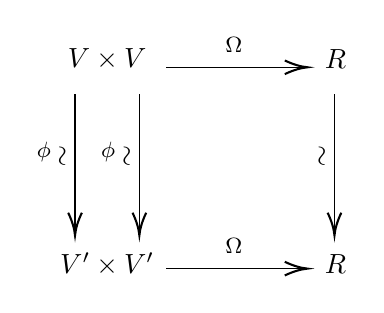
\begin{tikzpicture}[x=0.75pt,y=0.75pt,yscale=-1,xscale=1]
%uncomment if require: \path (0,300); %set diagram left start at 0, and has height of 300

%Straight Lines [id:da494304399766889] 
\draw    (280.5,80) -- (280.5,146) ;
\draw [shift={(280.5,148)}, rotate = 270] [color={rgb, 255:red, 0; green, 0; blue, 0 }  ][line width=0.75]    (10.93,-3.29) .. controls (6.95,-1.4) and (3.31,-0.3) .. (0,0) .. controls (3.31,0.3) and (6.95,1.4) .. (10.93,3.29)   ;
%Straight Lines [id:da03077396523282072] 
\draw    (155.5,80) -- (155.5,146) ;
\draw [shift={(155.5,148)}, rotate = 270] [color={rgb, 255:red, 0; green, 0; blue, 0 }  ][line width=0.75]    (10.93,-3.29) .. controls (6.95,-1.4) and (3.31,-0.3) .. (0,0) .. controls (3.31,0.3) and (6.95,1.4) .. (10.93,3.29)   ;
%Straight Lines [id:da8293026809275621] 
\draw    (186.5,80) -- (186.5,146) ;
\draw [shift={(186.5,148)}, rotate = 270] [color={rgb, 255:red, 0; green, 0; blue, 0 }  ][line width=0.75]    (10.93,-3.29) .. controls (6.95,-1.4) and (3.31,-0.3) .. (0,0) .. controls (3.31,0.3) and (6.95,1.4) .. (10.93,3.29)   ;
%Straight Lines [id:da4027318316111741] 
\draw    (199.5,67) -- (265.5,67) ;
\draw [shift={(267.5,67)}, rotate = 180] [color={rgb, 255:red, 0; green, 0; blue, 0 }  ][line width=0.75]    (10.93,-3.29) .. controls (6.95,-1.4) and (3.31,-0.3) .. (0,0) .. controls (3.31,0.3) and (6.95,1.4) .. (10.93,3.29)   ;
%Straight Lines [id:da5650396736156633] 
\draw    (199.5,164) -- (265.5,164) ;
\draw [shift={(267.5,164)}, rotate = 180] [color={rgb, 255:red, 0; green, 0; blue, 0 }  ][line width=0.75]    (10.93,-3.29) .. controls (6.95,-1.4) and (3.31,-0.3) .. (0,0) .. controls (3.31,0.3) and (6.95,1.4) .. (10.93,3.29)   ;

% Text Node
\draw (171,63) node    {$V\times V$};
% Text Node
\draw (171,162) node    {$V'\times V'$};
% Text Node
\draw (273.5,110) node  [rotate=-90]  {$\sim $};
% Text Node
\draw (148.5,110) node  [rotate=-90]  {$\sim $};
% Text Node
\draw (179.5,110) node  [rotate=-90]  {$\sim $};
% Text Node
\draw (232,56) node  [font=\footnotesize]  {$\Omega $};
% Text Node
\draw (232,153) node  [font=\footnotesize]  {$\Omega $};
% Text Node
\draw (281,63) node    {$\mathbb{R}$};
% Text Node
\draw (281,162) node    {$\mathbb{R}$};
% Text Node
\draw (140.5,108) node  [font=\footnotesize]  {$\phi $};
% Text Node
\draw (171.5,108) node  [font=\footnotesize]  {$\phi $};


\end{tikzpicture}
\end{figure}
\vspace{-1cm}

\begin{remark}
The requirement that $\phi$ is an isomorphism is not restrictive, since this is a simple consequence of the trivial kernel of $\Omega$.
\end{remark}

\begin{remark}
In the case of symplectic vector spaces, Theorem~\ref{th:decomp_th} says that every symplectic vector space of dimension $2n$ is symplectomorphic to $(\R^{2n},\Omega_0)$:
\begin{eqalign}
	(V, \Omega) \underset{\cat{Symp}}\iso (\R^{2n},\Omega_0)
\end{eqalign}
with $e_1,\dots,e_n,f_1,\dots,f_n$ the canonical basis of $\R^{2n}$ and $\Omega_0(e_i,e_j)=\Omega_0(f_i,f_j)=0$, $\Omega(e_i,f_j)=\delta_{ij}$, $\forall\,i,j=1,\dots,n$.\\
Notice that for spaces with non-degenerate symmetric form (Riemannian spaces) the situation is different, since in $\R^n$ we can define several metrics that differs only by them signature, i.e. each Riemann space $(V,g)$ is isomorphic to a "canonical" space $(\R,g_0)$ with
\begin{eqalign}
g_0=\begin{pmatrix}I_k&0\\0&-I_{n-k}\end{pmatrix}
\end{eqalign}
for some value of $k\neq n$. 
\end{remark}

\section{Symplectic manifolds}
Endowing the tangent bundle of a manifold with a symplectic structure, we get the differential analogue of a symplectic vector space:

\begin{definition}
	A \textbf{symplectic form} $\omega$ on a smooth manifold $M$ is a non-degenerate\footnotemark, closed, differentiable $2$-form on $M$. A \textbf{symplectic manifold} is a manifold $M$ equipped with a symplectic form on $M$.
	\footnotetext{In this context, non-degenerate means pointwise non-degenerate.}
\end{definition}

Therefore at each point $p \in M$ the tangent space $T_pM$ is a symplectic vector space with symplectic form $\omega_p$.

\begin{example}
\label{ex:eu_sp_sphere}
	\leavevmode
	\begin{enumerate}
		\item Any Euclidean space $\R^{2n}$ can be equipped with the following form
		\begin{eqalign}
			\omega_0 = \sum_{i=1}^n dx^i \wedge dy^i
		\end{eqalign}
		where we call $y^i$ the coordinate $x^{n+i}$. With this definition $\omega_0$ is, pointwise, the form $\Omega_0$ discussed previously. Moreover, it is closed as
		\begin{eqalign}
			d\omega_0 &= \sum_{i=1}^n d(dx^i \wedge dy^i)\\
			&= \sum_{i=1}^n d^2x^i \wedge y^i - dx^i \wedge d^2y^i = 0
		\end{eqalign}
		\item The $2$-sphere is a symplectic manifold. Indeed, consider its immersion in $\R^3$ defined as $S^2 = \{ x \in \R^3 \suchthat \|x\| = 1\}$. Then
		\begin{eqalign}
			T_xS^2 = \{ v \in \R^3 \suchthat \langle v, x \rangle = 0 \}
		\end{eqalign}
		can be made into a symplectic vector space by means of
		\begin{eqalign}
			\omega_x (u,v) := \langle x, u \times v \rangle, \quad \forall u,v \in T_xS^2.
		\end{eqalign}
		which trivially defines a differential form $\omega \in \Omega^2(S^2)$. Finally, since $\dim S^2 = 2$, the form $\omega$ is necessarily closed.
	\end{enumerate}
\end{example}

Since $\dim T_pM = \dim M$, $M$ inherits the condition on the dimension of $T_pM$: $M$ must be even-dimensional. However this time, even-dimensionality is not a sufficient condition for a manifold to be symplectic. A further necessary condition is given by the following theorem.

\begin{theorem}
\label{th:symp_vol_form}
	Let $(M, \omega)$ be a symplectic manifold, with $\dim M = 2n$. Then the $n$-th exterior power of $\omega$ is a volume form.
\end{theorem}
\begin{proof}
	The rank of $\omega^{\wedge n}$ is $2n$, so the claim makes sense. Choose $p \in M$ now, and fix a local frame $E_1, \ldots, E_n, F_1, \ldots, F_n$ around $p$ in such a way that  it is in $p$ a canonical basis as per Theorem~\ref{th:decomp_th}. Then:
	\begin{eqalign}
		\omega^{\wedge n}_p (E_1\vert_p, \ldots, E_n\vert_p, F_1\vert_p, \ldots, F_n\vert_p) &= \omega_p(E_1\vert_p, F_1\vert_p) \cdot \ldots \cdot \omega_p(E_n\vert_p, F_n\vert_p) = 1
	\end{eqalign}
	thus the form is everywhere positive.
\end{proof}
\begin{corollary}
	If $M$ is symplectic, it is orientable.
\end{corollary}

The obvious remark is then that non-orientable manifolds can't be symplectic even in the even-dimensional case; e.g. the projective plane does not admit a symplectic structure.

Other obstructions are given by topology. For example

\begin{theorem}
	The $2$-sphere is the only sphere admitting a symplectic structure.
\end{theorem}
\begin{proof}
	In Example~\ref{ex:eu_sp_sphere} we exhibited a symplectic structure for $S^2$, so only we need to prove any $S^{2n}$ with $n \geq 2$ does not admit one. Let $\omega \in \Omega^2(S^{2n})$ be a closed form. Recall $H^2_dr(S^{2n}) = 0$, as the only non-vanishing homologies (hence cohomologies by de Rham's Theorem) are the bottom and the top ones and we assumed $n > 1$. By definition of cohomology, this means all closed $2$-forms are automatically exact, implying there exists an $\eta \in \Omega^1(S^{2n})$ such that $d\eta = \omega$. Hence, using Corollary~\ref{cor:ext_power_is_exact} and Stokes' Theorem:
	\begin{eqalign}
		\int_{S^{2n}} \omega^{\wedge n} = \int_{S^{2n}} d\eta = \int_{\partial S^{2n}} \eta = 0
	\end{eqalign}
	Then, by Theorem~\ref{th:symp_vol_form}, it must be $\omega = 0$ thus not symplectic.
\end{proof}

\begin{remark}
	Notice \textbf{the proof can be generalized to any compact manifold with vanishing second cohomology}. Moreover, it shows a symplectic form cannot be exact on a compact manifold.
\end{remark}

\begin{definition}
	A submanifold $N$ of a symplectic manifold $(M, \omega)$ is a \textbf{symplectic submanifold} if $(N, \omega\vert_N)$ is symplectic.
\end{definition}
\begin{definition}
	A smooth map $\phi : M \to N$, where $M$ and $N$ are symplectic manifolds with symplectic forms $\omega$ and $\eta$ respectively, is called a \textbf{symplectomorphism} if it is an embedding and
	\begin{eqalign}
		\phi^* \eta = \omega
	\end{eqalign}
\end{definition}

\begin{remark}
\label{rmk:inverse_ipr}
	As with symplectic vector spaces, a symplectic form induces a natural isomorphism of $\fields(M)$ with $\Omega^1(M)$, which is the extension of the pointwise isomorphism $\tilde\omega_p : T_pM \to T^*_pM$, defined as before by partial application:
	\begin{eqalign}
		\omega : \fields(M) &\longto \Omega^1(M)\\
				X &\longmapsto \ipr{X}\omega
	\end{eqalign}
	The inverse map is
	\begin{eqalign}
		\omega^{-1} : \Omega^1(M) &\longto \fields(M)
	\end{eqalign}
	and it is defined as to satisfy
	\begin{eqalign}
		\omega^{-1}(\ipr{X}\omega) = X.
	\end{eqalign}
\end{remark}

\subsection[The canonical symplectic structure on the cotangent bundle]{The canonical symplectic structure\\on the cotangent bundle}
The chief example of symplectic manifolds are cotangent bundles of smooth manifolds. In fact, there's a natural/canonical way to equip $M= T^*X$ with a symplectic structure. Notice that $\dim T^*X = 2\dim X$ so that, in principle, we can expect to assign a symplectic structure to arbitrary cotangent bundles. Clearly, as we've seen, dimensionality isn't the only obstruction so we need to exhibit a symplectic form.

The construction of the symplectic structure exploits a particular, naturally defined, $1$-form on $T^*X$. The symplectic form will then be it's exterior derivative.

\begin{construction}
	Let $\pi : T^*X \to X$ be the bundle projection. Notice that a differential $1$-form on $T^*X$ is a function $T^*X \to T^*T^*X$ (with the additional condition of being compatible with the fibers, more on this later) which is exactly the type of function $d\pi^*$ is. If we unpack its definition from Construction~\ref{const:global_diff_and_dual}, we get
	\begin{eqalign}
		d\pi^* : T^*X &\longto T^*T^*X\\
		(x, \xi) &\longmapsto (\pi^{-1}(x),\, \xi \circ d\pi_{\pi^{-1}(x)})
	\end{eqalign}
	So the definition fails. We already knew this: we remarked that $dF^*$ is well-defined if and only if $F$ is a diffeomorphism, which is certainly not the case for $\pi$. On the other hand, we can try to fix this pathology by finding another way to choose a ``canonical'' element from $\pi^{-1}(x)$ in the mapping expression of $d\pi^*(x, \xi)$. Indeed, since $\pi$ is surjective, that's the only obstruction! And we clearly see that those $\pi^{-1}(x)$ can be unambiguously resolved by simply using the argument of the sought function. So we define the mapping
	\begin{eqalign}
		\alpha : T^*X &\longto T^*T^*X\\
		(x, \xi) &\longmapsto ((x, \xi), \xi \circ d\pi_{(x, \xi)})
	\end{eqalign}
	or, using the fiberwise duals (Construction~\ref{const:dual_diff_at_P}):
	\begin{eqalign}
		\alpha(x, \xi) = d\pi^*_{(x, \xi)} \xi.
	\end{eqalign}
	This is clearly well-defined as the domain of $d\pi^*_{(x,\xi)}$ is precisely $T^*_{(x,\xi)} T^*X$. The $1$-form we just defined is called \textbf{Liouville form} or \textbf{tautological one-form}.
\end{construction}

The name \emph{tautological} comes from the following property: for every $\mu \in \Omega^1(X)$,
\begin{eqalign}
	\mu^* \alpha = \mu
\end{eqalign}
where $\mu^*$ is the pullback of $\mu$ when seen as smooth map $X \to T^*X$.

Let's compute what this form looks like, fixing coordinates on the involved spaces. Notice, first, that coordinates on $X$ suffice to fix relevant coordinates on both $T^*X$ and $T^*T^*X$, by using the induced reference frames as bases for the fibers:

\begin{center}
	\begin{tabular}{c|l|l}
		\textbf{Space} & \textbf{Local frame} & \textbf{Coordinates}\\[1ex]
		\hline
		$X$ & \textcolor{gray}{(does not apply)} & $(x^1, \ldots, x^n)$\\[1ex]
		$T^*X$ & $(dx^1, \ldots, dx^n)$ & $(x^1, \ldots, x^n, \xi^1, \ldots, \xi^n)$\\[1ex]
		$T^*T^*X$ & $(dx^1, \ldots, dx^n, d\xi^1, \ldots, d\xi^n)$ & $(x^1, \ldots, x^n, \xi^1, \ldots, \xi^n, \chi^1, \ldots, \chi^{2n})$\\
	\end{tabular}
\end{center}

Basically, for $T^*X$ and $T^*T^*X$, the second half of the coordinates are just the components with respect to the local frame on their left\footnote{This is doable for any locally trivial vector bundle: any point $y \in E$ of a vector bundle $\pi: E \to M$ can be thought as a pair $(\pi(y), v)$ so that we use the coordinates of $M$ for the first component, and components with respect to the local frame induced by the coordinates of $M$ on $E_{\pi(y)}$ for the second.}.

When we focus on a single fiber \textbf{half of the coordinates become superfluous since are fixed by the choice of fiber}. Therefore a covector $\xi \in T^*_x X$ will be written as
\begin{eqalign}
	\xi = \xi_j(x) dx^j\vert_x,
\end{eqalign}
while $\chi \in T^*_{(x,\xi)} T^*X$ (a double covector?) as
\begin{eqalign}
	\chi = \chi_j(x,\xi) dx^j\vert_{(x,\xi)} + \chi_{j+n}(x,\xi) d\xi^j\vert_{(x,\xi)}.
\end{eqalign}

In this setting, $\pi : T^*X \to X$ is the following map
\begin{eqalign}
	\pi(x, \xi) = \pi(x^1, \ldots, x^n, \xi^1, \ldots, \xi^n) = (x^1, \ldots, x^n), \quad \forall (x,\xi) \in T^*X
\end{eqalign}
whose differential, expressed as its Jacobian matrix, is then
\begin{eqalign}
	d\pi_{(x, \xi)} = \begin{pmatrix}
		\partial_i \pi^j
	\end{pmatrix}\rvert_{(x, \xi)} = \begin{pmatrix}
		\bigpder{\pi^j}{x^i} & \bigpder{\pi^j}{\xi^i}
	\end{pmatrix}\rvert_{(x, \xi)} = \begin{pmatrix}
		I_n & 0
	\end{pmatrix}.
\end{eqalign}
Then
\begin{eqalign}
	\alpha(x, \xi) &= d\pi^*_{(x, \xi)}\xi = \xi \circ d\pi_{(x, \xi)} = \xi_j \cancelto{\delta^j_k}{\pder{\pi^j}{x^k}} dx^k\vert_{(x,\xi)} + \xi_j \cancelto{0}{\pder{\pi^j}{\xi^k}} d\xi^k\vert_{(x,\xi)} = \xi_k dx^k\vert_{(x,\xi)}
\end{eqalign}

The ``canonicity'' of $\alpha$ is also witnessed by the following fact:

\begin{theorem}
\label{th:canonicity_of_taut}
	Let $F : X_1 \isoto X_2$ be a diffeomorphism and $\alpha, \beta$ the Liouville forms respectively on $X_1$ and $X_2$. Call $\mathcal{F}$ the dual morphism induced by $F^{-1}$. Then $\mathcal F^* \beta = \alpha$.
	\begin{diagram}
	\label{diag:liouville}
		T^*X_1 \arrow{d}{\pi_1} \arrow{r}{\mathcal F} \& T^*X_2 \arrow{d}{\pi_2}\\
		X_1 \arrow{r}{F} \& X_2
	\end{diagram}
\end{theorem}
\begin{proof}
	For each $(x, \xi) \in T^*X_2$,
	\begin{eqalign}
		\mathcal{F}(x, \xi) = (F(x), d(F^{-1})^*_{(x,\xi)}\xi),
	\end{eqalign}
	so that
	\begin{eqalign}
		(\mathcal F^* \beta)_{(x, \xi)} &= \beta_{\mathcal{F}(x, \xi)} \circ d{\mathcal F}_{(x, \xi)}\\
		&=  d(F^{-1})^*_{(x,\xi)} \xi \circ d(\pi_2)_{\mathcal F(x,\xi)} \circ d(d(F^{-1})^*)_{(x, \xi)}\\
		&= \xi \circ d(F^{-1})_{(x,\xi)} \circ d(\pi_2 \circ d(F^{-1})^*)_{(x, \xi)} \comment{by chain rule}\\
		&= \xi \circ d(F^{-1})_{(x,\xi)} \circ d(F \circ \pi_1)_{(x, \xi)} \comment{by Diagram~\ref{diag:liouville}}\\
		&= \xi \circ d(\pi_1)_{(x, \xi)}\\
		&= d(\pi_1)^*_{(x, \xi)} \xi = \alpha_{(x,\xi)};
	\end{eqalign}
	which amounts to the thesis.
\end{proof}

\begin{definition}
	The \textbf{canonical symplectic form} on $T^*X$ is
	\begin{eqalign}
		\omega = -d\alpha
	\end{eqalign}
\end{definition}

Notice the minus sign, that's unavoidable and rigs pretty much all symplectic geometry.

With the same coordinates we used before, $\omega$ is
\begin{eqalign}
	\omega &= -d\alpha\\
	&= - d(\xi_j dx^j)\\
	&= - d\xi_j \wedge dx^j - \xi_j \wedge \cancelto{0}{d^2x^j} = \sum_{j=1}^n d\xi^j \wedge dx^j
\end{eqalign}

\section{Symplectomorphisms and Lagrangian manifolds}
Theorem~\ref{th:canonicity_of_taut} says the pullback of $(f^{-1})^* : T^*X_1 \to T^*X_2$ is a symplectomorphism. In particular, when $X=X_1=X_2$, there's a natural morphism of groups,
\begin{diagram}
	\Diff(X) \arrow[hookrightarrow]{r} \& \Symp(T^*X, \omega),
\end{diagram}
whose domain is the group of diffeomorphisms of $X$ and whose codomain is the group of symplectomorphisms of $(T^*X, \omega)$. Recall that $X$ lives inside $T^*X$ as its zero section, thus the morphism is actually an inclusion, justifying its depiction by an hooked arrow. However, this map is not onto, since not all symplectomorphism arise in this way: for instance, translation along fibers of $T^*X$ is not in the image.

This leaves us with the problem of finding these additional symplectomorphisms. If diffeomorphisms of the base space are too few to induce all of them, conversely diffeomorphisms of the total space are too many and we need to weed out all the ones which aren't preserving the symplectic structure.

Luckily, a new geometric concept comes to help:

\begin{definition}
	A submanifold $Y$ of a symplectic manifold $(M, \omega)$ is called \textbf{Lagrangian} when
	\begin{enumerate}
		\item $\dim Y = \frac12 \dim M$ and
		\item $Y$ is \textbf{isotropic}, i.e. if $\iota: Y \into M$ is the embedding of $Y$, then $\iota^* \omega = 0$
	\end{enumerate}
\end{definition}

These submanifolds are closely related to symplectomorphisms. A first hint comes from the following result.

\begin{exercise}
\label{ex:lagrangian_submanifolds_of_cotangent_bundles}
	Let $M = T^*X$ for a smooth manifold $X$, along with its canonical symplectic structure. Prove the graph of $\alpha \in \Omega^1(X)$ defines a Lagrangian submanifold of $M$ if and only if $\alpha$ is closed, that is $d\alpha =0$.
\end{exercise}
\begin{proof}
	Indeed, let $\Gamma$ be the graph of $\alpha$. Then $\Gamma$ is trivally an embedded submanifold of $M$ of dimension $\frac12 \dim M$. Fix now coordinates as in the construction of Liouville's form. For the isotropy condition, a quick computation gives
	\begin{eqalign}
		d\iota = \begin{pmatrix}
			\delta^i_j & 0\\
			\partial_j \alpha_i & 0
		\end{pmatrix}
	\end{eqalign}
	from which
	\begin{eqalign}
		\iota^* \omega &= \sum_{j=1}^n \iota^* dx^j \wedge \iota^* d\xi^j = \sum_{j=1}^n \delta^i_j dx^j \wedge (\partial_j \alpha_i) dx^j = -d\alpha
	\end{eqalign}
	giving the claim.
\end{proof}

Consider now two symplectic manifolds $(M_1,\omega_1)$ and $(M_2, \omega_2)$, with the same dimension $\dim M_1 = \dim M_2$. We can endow $M_1 \times M_2$ with two different symplectic structures
\begin{eqalign}
	\omega_\pm = \pr_1^*\omega_1 \pm \pr_2^*\omega_2
\end{eqalign}
where $\pr_.$ denote a projection map.

\begin{theorem}
\label{th:char_of_symplectomorphism}
	A diffeomorphism $\phi : M_1 \to M_2$ is a symplectomorphism if and only if its graph submanifold
	\begin{diagram}
		\Gamma_\phi = \{(p, \phi(p)) \suchthat p \in M_1\} \arrow[hookrightarrow]{r}{\iota} \& M_1 \times M_2
	\end{diagram}
	is Lagrangian with respect to $\omega_-$.
\end{theorem}
\begin{proof}
	As $\dim M_1 = \dim M_2$ (because they're diffeomorphic through $\phi$),
	\begin{eqalign}
		\dim \Gamma_\phi = \dim M_1 = \frac12 \dim (M_1 \times M_2).
	\end{eqalign}
	Moreover, We have
	\begin{eqalign}
		\iota^*\omega_- = \iota^*\pr_1^* \omega_1 - \iota^*\pr_2^* \omega_2 = (\pr_1 \circ \iota)^* \omega_1 - (\pr_2 \circ \iota)^* \omega_2
	\end{eqalign}
	Since $\iota$ sends $p \mapsto (p,\phi(p))$, composing with the projection on the first component yields $\id_{M_1}$, and composing with the other projection yields $\phi$. Thus
	\begin{eqalign}
		\iota^*\omega_- = \id^*\omega_1 - \phi^*\omega_2
	\end{eqalign}
	Implying
	\begin{eqalign}
		\phi^*\omega_2 = \omega_1 \iff \iota^*\omega_- = 0
	\end{eqalign}
	which is the claim we wanted to prove.
\end{proof}

\begin{remark}
	The theorem \emph{does not} state any Lagrangian submanifold is the graph of a symplectomorphism: it is assumed, a fortiori, that $\phi$ is a diffeomorphism.
\end{remark}

This result, combined with Exercise~\ref{ex:lagrangian_submanifolds_of_cotangent_bundles}, gives us a systematic way to produce symplectomorphisms of a cotangent space.

\begin{construction}
	In the case $M_1 = T^*X_1$ and $M_2 = T^*X_2$, along with their canonical symplectic structure, then
	\begin{eqalign}
		T^*X_1 \times T^*X_2 = T^*(X_1 \times X_2)
	\end{eqalign}
	and the space is symplectic with symplectic form
	\begin{eqalign}
		\omega_- = - d(\pr_1^*\alpha_1 - \pr_2^*\alpha_2).
	\end{eqalign}
	On the other hand, the canonical symplectic form on $T^*(X_1 \times X_2)$ is
	\begin{eqalign}
		\omega_+ = - d(\pr_1^*\alpha_1 + \pr_2^*\alpha_2)
	\end{eqalign}
	By Exercise~\ref{ex:lagrangian_submanifolds_of_cotangent_bundles}, we know how to construct Lagrangian manifolds on $T^*(X_1 \times X_2)$ with respect to its canonical symplectic structure as cotangent bundle. However, Theorem~\ref{th:char_of_symplectomorphism} refers to the other symplectic structure of $T^*(X_1 \times X_2)$, obtained from its product structure. Thus we leverage the following procedure:
	\begin{enumerate}
		\item Produce a Lagrangian submanifold of $T^*(X_1 \times X_2)$ with respect to $\omega_+$: choose any function $f \in \Cinfty(X_1 \times X_2)$ and consider $\Gamma_{df} = \{(x,y,d_x f, d_y f) \suchthat (x,y) \in X_1 \times X_2\}$.
		\item Twist the graph to $\tilde\Gamma_{df} = \{(x,y,d_xf,-d_yf) \suchthat (x,y) \in X_1 \times X_2\}$ (because the only difference between $\omega_+$ and $\omega_-$ is exactly this twist on the second factor) to get a Lagrangian submanifold with respect to $\omega_-$.
		\item For $\tilde\Gamma_{df}$ to be the graph of a diffeomorphism $\phi : T^*X_1 \isoto T^*X_2$, it needs to satisfy a local condition: it must not be ``vertical'' at any point on the $T^*X_1$-$T^*X_2$ plane, that is, the projection $\pr_1 : \tilde\Gamma_{df} \to T^*X_1$ must have no critical points. This means
		\begin{eqalign}
			\det \left( \spder{f}{y^j}{x^i} \right) \neq 0
		\end{eqalign}
		If this is satisfied, then $\phi$ sends the first and third component of a point in $\tilde\Gamma_{df}$ to the second and fourth components:
		\begin{eqalign}
			\phi : (x,\xi) \mapsto (y,\eta)
		\end{eqalign}
		where
		\begin{eqalign}
		\label{eq:canonical_transf_from_gen_funcs}
			\begin{cases}
				\xi_i = \bigpder{f}{x^i}(x,y)\\
				\eta_i = -\bigpder{f}{y^i}(x,y)
			\end{cases}
		\end{eqalign}
	\end{enumerate}
\end{construction}

Eventually, in the case $X_1 = X_2 = X$, we just explained geometrically how \textbf{canonical transformations} of a phase-space manifold arise from \textbf{generating functions} $f \in \Cinfty(X \times X)$.

\section{Darboux's Theorem}
We'll now pursue a local description of symplectic manifolds. For this section, refer to \cite[Section 1.4]{cannas2005symplectic} and \cite[Section 1.5]{cannas2005symplectic}.

\subsection{Tubular neighbourhoods}
\begin{definition}
	Given a closed embedding ${\iota : X \into M}$ of a $k$-dimensional submanifold $X$ into its $n$-dimensional ambient manifold $M$, its \textbf{normal bundle} is
	\begin{eqalign}
		NX := TM/TX
	\end{eqalign}
	defined pointwise on $X$.
\end{definition}

\begin{definition}
	A \textbf{tubular neighbourhood} of $X$ is an open neighbourhood $U$ of $\iota(X)$ in $M$ diffeomorphic to a convex\footnotemark\ neighbourhood $U_0 \subseteq NX$ of the zero section of the normal bundle.
	\footnotetext{In a vector space, a subset is convex if any convex combination of elements of the subset is still in the subset.}
\end{definition}

The convexity condition means that $U_0 \cap N_xX$ has to be convex as a subset of the vector space $N_x X$.

Hence the situation is the following:
\begin{diagram}
	NX \arrow[relation=\supseteq]{r} \&[-3ex] U_0 \arrow[shift left]{dr}{\pi_0} \arrow{rr}{\phi} \& \& \arrow[dashed, shift left]{dl}{\pi} U \arrow[relation=\subseteq]{r} \&[-3ex] M\\
	\& \& X \arrow[hookrightarrow, shift left]{ur}{\iota} \arrow[hookrightarrow, shift left]{ul}{\iota_0}
\end{diagram}
where $\pi_0$ is the bundle morphism, $\phi$ is the diffeomorphism we ask for in the definition and $\pi$ arises from commutativity of the diagram.

\paragraph{Topological properties of tubular neighbourhoods.} The choice of properties of a tubular neighbourhood is tuned as to make it a very useful tool to probe the de Rham cohomology of $X$. From \ref{par:ind_maps_on_de_rham} we know two spaces have the same cohomology when they are homotopically equivalent. Indeed, notice $\pi\iota = \id_X$ already. On the other hand we clearly don't have $\iota\pi = \id_U$. However, $\iota\pi$ is still homotopic to the identity, thanks to the convexity condition on $U_0$. In fact $U_0$ is just a fattening of $X$ and diffeomorphic to $U$, so that $U$ contracts to $X$ as well. In this way $\id \homtop \iota\pi$. Then $(\iota\pi)^* = \pi^*\iota^* = \id_U^* : H^k_{dR}(U) \to H^k_{dR}(U)$. Hence, \textbf{$\pi^*$ is an isomorphism of de Rham cohomology groups}, which means
\begin{eqalign}
	H^k_{dR}(U) \iso H^k_{dR}(X).
\end{eqalign}

\subsection{Moser's theorems}
\begin{theorem}[Moser's First Theorem]
\label{th:first_moser_th}
	Let $(M, \omega_t = (1-t)\omega_0+t\omega_1)$ be a symplectic \textbf{compact} manifold for each $t \in [0,1]$, and $\overline{\omega_0} = \overline{\omega_1} \in H^2_{dR}(M)$. Then there exists $\rho: M \times \R \to M$ such that $\rho_t : (M, \omega_t) \isoto (M,\omega_0)$ is a symplectomorphism for all $t \in [0,1]$.
\end{theorem}

The idea is that if you have a ``flowing'' symplectic structure, you can compensate by a ``flowing'' change of coordinates. This is given by a one-parameter group of diffeomorphisms, hence by the flow of a vector field on $M$. In this vein, the theorem is basically equivalent to the following:

\begin{lemma}[Moser's trick]
	Under the assumptions of Moser's First Theorem, there exists $V_t \in \fields(M)$ depending smoothly on $t$ and such that
	\begin{eqalign}
		\Lie{V_t}\omega_t+\der{\omega_t}{t}=0.
	\end{eqalign}
\end{lemma}
\begin{proof}
	Notice that $\der{}{t} \omega_t = \omega_1-\omega_0$, and since $\omega_1$ and $\omega_0$ are cohomologous, their difference is cohomologous to $\overline 0 \in H^2_{dR}(M)$. This means that $\omega_1 -\omega_0 = d\mu$ for some $\mu \in \Omega^1(M)$. Moreover, by Cartan's magic formula
	\begin{eqalign}
		\Lie{V_t}\omega_t = d \ipr{V_t}\omega_t + \cancel{\ipr{V_t}d\omega_t}.
	\end{eqalign}
	Hence the equation we want to prove has been reduced to
	\begin{eqalign}
		d(\ipr{V_t}\omega_t + \mu) = 0
	\end{eqalign}
	which of course holds in particular if $\ipr{V_t}\omega_t = -\mu$ (\textbf{Moser's equation}), i.e. when
	\begin{eqalign}
		V_t = -\omega_t^{-1}(\mu).
	\end{eqalign}
\end{proof}

\begin{proof}[Proof of Moser's Theorem (\ref{th:first_moser_th})]
	Let $\rho_t$ be a flow as claimed. Then if $V_t$ is the vector field associated to it (i.e. its derivative\footnotemark), we can write
	\begin{eqalign}
	\label{eq:der_of_flowing_symp}
		\der{}{t}(\rho_t^*\omega_t) = \rho_t^*\left(\Lie{V_t}\omega_t + \der{\omega_t}{t}\right).
	\end{eqalign}
	Then we see that, as $M$ is compact, we could reverse the argument and get all of $\rho_t$ by integration of $V_t$, which is given to us by Moser's trick.
\end{proof}
\footnotetext{We have to be careful about the meaning of the parameter $t$! There are two different ``times'' to consider in a similar flow, indeed, $\rho_t$ satisfies the following ODE:
\begin{eqalign}
	V_t = \der{}{s} (\rho_s\rho_t^{-1})\vert_{s=t}
\end{eqalign}
It's like an usual flow in which vectors, however, change with time (\emph{non-autonomous flow}), so at time $t$ the curve has tangent vector $V_t$. For comparison, this is the equation in the \emph{autonomous} (i.e. the field doesn't vary with time) case:
\begin{eqalign}
	V = \der{}{s} \rho_s \vert_{s=0}.
\end{eqalign}}

\begin{remark}
	Moser's Theorem can be proved also in the more general case where $\omega_t$ is a continuous curve inside a single cohomology class, that is
	\begin{eqalign}
		\der{}{t} \overline{\omega_t} = \overline 0 \in H^2_{dR}(M).
	\end{eqalign}
	A simple application of this is that if $(M, \omega)$ is symplectic and $\eta \in \Omega^1(M)$, then $(M, \omega + d\eta)$ is symplectic as well and symplectomorphic to the original manifold.
\end{remark}

\begin{theorem}[Moser's Relative Theorem]
	Let $(M, \omega_0)$ and $(M, \omega_1)$ be two symplectic structures on $M$, $\iota : X \into M$ a closed embedding of a compact submanifold such that
	\begin{eqalign}
		\omega_0\vert_p = \omega_1\vert_p, \quad \forall p \in X
	\end{eqalign}
	Then there are neighbourhoods $U_0$ and $U_1$ of $\iota(X)$ and a symplectomorphism $\phi: U_0 \isoto U_1$, which on $X$ restricts to the identity, such that
	\begin{diagram}
		(U_0, \omega_0) \arrow{rr}{\phi} \& \& (U_1, \omega_1)\\
		\& X \arrow[hookrightarrow]{ul}{\iota_0} \arrow[hookrightarrow, swap]{ur}{\iota_1}
	\end{diagram}
\end{theorem}
\begin{proof}
	Choose a tubular neighbourhood $U_0$ of $X$. Again, under the given assumptions on $\omega_0$ and $\omega_1$, $\omega_1\vert_{U_0}-\omega_0\vert_{U_0} = d\mu$ for $\mu \in \Omega^1(U_0)$. Let $\omega_t := \omega_0 + t(\omega_1-\omega_0) = \omega_0 + td\mu$. This is symplectic for generic $t \in [0,1]$, hence shrinking $U_0$ if necessary we can assume $\omega_t$ is symplectic on $U_0$.

	To see the shrunk neighbourhood does not degenerate, notice that
	\begin{eqalign}
		\{(p,t) \in M \times [0,1] \suchthat \det \omega_t(p) = 0\}
	\end{eqalign}
	is closed. Same for $\iota(X) \times [0,1]$. Then as the two do not intersect, they can be separated by an open neighbourhood around $\iota(X) \times [0,1]$, whose projection on the first factor contains a tubular neighbourhood.

	Solve now Moser's equation in this neighbourhood. We get then a flow $\rho_t : U_0 \times [0,1] \to M$ which carries $\omega_t$ to $\omega_0$ for each $t \in [0,1]$. To see we proved the theorem, set $\phi = \rho_1$ and $U_1 = \rho_1(U_0)$. Since $\omega_1 \vert_{\iota(X)} = \omega_0\vert_{\iota(X)}$ we have $\rho_t\vert_X = \id_X \ \forall t$, hence in particular for $\rho_1 = \phi$, concluding the proof.
\end{proof}

\begin{theorem}[Darboux]
	Let $(M, \omega)$ be a symplectic manifold and $p \in M$. Then there exist a chart $(U, (x^1, \ldots, x^n, y^1, \ldots, y^n))$ around $p$ such that, on $U$
	\begin{eqalign}
		\omega = \sum_{i=1}^n dx^i \wedge dy^i.
	\end{eqalign}
\end{theorem}
\begin{proof}
	Fix a symplectic basis for $(T_pM, \omega_p)$ (following the procedure given in Theorem~\ref{th:decomp_th}) so that $\omega_p = \sum_{i=1}^n {dx^i}'\vert_p \wedge {dy^i}'\vert_p$ in those coordinates. By triviality of the tangent bundle, these coordinates are actually valid in a whole open neighbourhood $U'$ of $p$, so that around $p$ we get to define a symplectic form $\omega' = \sum_{i=1}^n {dx^i}' \wedge {dy^i}'$. Then by Moser's Relative Theorem applied to $X=\{p\}$, $\omega$ is equivalent to $\omega'$ on a neighbourhood $U_1 \cap U'$ of $p$, thanks to a diffeomorphism $\phi : U_0 \to U_1$. Hence setting $x^i = {x^i}' \circ \phi$, $y^i = {y^i}' \circ \phi$, we are done.
\end{proof}

\begin{remark}
	The three theorems exposed in this section form a hierarchy of results about symplectomorphisms of $(M, \omega)$ fixing an immersed symplectic compact submanifold $(X, \omega')$. Moser's Theorem addresses the case $X=M$, Darboux's Theorem addresses the case $X=\{\bullet\}$ and Moser's Relative Theorem addresses any other case in-between (be careful about the little differences between the three theorems, though).
\end{remark}

\begin{remark}
	What can we say about the different symplectic structures a manifold admits? Are they all symplectomorphic? A different yet related question is: \textbf{are there some invariants which can discern between non-equivalent symplectic structures?} Gromov proved a result stating that $\Symp(M, \omega)$ (the group of symplectomorphisms of $(M, \omega)$) is either dense or closed in $\Diff(M)$ (\emph{Gromov's alternative}). In the first case, it would have meant that symplectic topology is undistinguishable from differential topology, yet it was later proved that the second case holds, so that there is interest in studying the symplectic structures of a manifold. However, this no easy task. In fact, Darboux's theorem tells us \textbf{symplectic structures have no local invariants}: to distinguish them you have to look at global data, which is harder to work with. For example, we'll immediately see in the next chapter that a very intuitive cohomology theory fails to classify symplectic structures (while its later extension to Poisson structures partially succeed to do this). An algebraic invariant which accomplish this is called \textbf{Floer cohomology}, and requires more machinery than what we'll see here.
\end{remark}

\end{document}